%%
%% This is file `sample-manuscript.tex',
%% generated with the docstrip utility.
%%
%% The original source files were:
%%
%% samples.dtx  (with options: `manuscript')
%% 
%% IMPORTANT NOTICE:
%% 
%% For the copyright see the source file.
%% 
%% Any modified versions of this file must be renamed
%% with new filenames distinct from sample-manuscript.tex.
%% 
%% For distribution of the original source see the terms
%% for copying and modification in the file samples.dtx.
%% 
%% This generated file may be distributed as long as the
%% original source files, as listed above, are part of the
%% same distribution. (The sources need not necessarily be
%% in the same archive or directory.)
%%
%% Commands for TeXCount
%TC:macro \cite [option:text,text]
%TC:macro \citep [option:text,text]
%TC:macro \citet [option:text,text]
%TC:envir table 0 1
%TC:envir table* 0 1
%TC:envir tabular [ignore] word
%TC:envir displaymath 0 word
%TC:envir math 0 word
%TC:envir comment 0 0
%%
%%
%% The first command in your LaTeX source must be the \documentclass command. This is the generic manuscript mode required for submission and peer review.
\documentclass[manuscript,screen,review]{acmart}
%% To ensure 100% compatibility, please check the white list of
%% approved LaTeX packages to be used with the Master Article Template at
%% https://www.acm.org/publications/taps/whitelist-of-latex-packages 
%% before creating your document. The white list page provides 
%% information on how to submit additional LaTeX packages for 
%% review and adoption.
%% Fonts used in the template cannot be substituted; margin 
%% adjustments are not allowed.

%%
%% \BibTeX command to typeset BibTeX logo in the docs
\AtBeginDocument{%
  \providecommand\BibTeX{{%
    \normalfont B\kern-0.5em{\scshape i\kern-0.25em b}\kern-0.8em\TeX}}}

%% Rights management information.  This information is sent to you
%% when you complete the rights form.  These commands have SAMPLE
%% values in them; it is your responsibility as an author to replace
%% the commands and values with those provided to you when you
%% complete the rights form.
%\setcopyright{acmcopyright}
%\copyrightyear{2023}
%\acmYear{2023}

%% These commands are for a PROCEEDINGS abstract or paper.
% \acmConference[Conference acronym 'XX]{Make sure to enter the correct
%   conference title from your rights confirmation emai}{June 03--05,
%   2018}{Woodstock, NY}
%
%  Uncomment \acmBooktitle if th title of the proceedings is different
%  from ``Proceedings of ...''!
%
%\acmBooktitle{Woodstock '18: ACM Symposium on Neural Gaze Detection,
%  June 03--05, 2018, Woodstock, NY} 

%% These commands are for a JOURNAL article.
%\acmJournal{JACM}
%\acmVolume{37}
%\acmNumber{4}
%\acmArticle{111}
%\acmMonth{8}

%\acmPrice{15.00}
%\acmISBN{978-1-4503-XXXX-X/18/06}


%%
%% Submission ID.
%% Use this when submitting an article to a sponsored event. You'll
%% receive a unique submission ID from the organizers
%% of the event, and this ID should be used as the parameter to this command.
%%\acmSubmissionID{123-A56-BU3}

%%
%% For managing citations, it is recommended to use bibliography
%% files in BibTeX format.
%%
%% You can then either use BibTeX with the ACM-Reference-Format style,
%% or BibLaTeX with the acmnumeric or acmauthoryear sytles, that include
%% support for advanced citation of software artefact from the
%% biblatex-software package, also separately available on CTAN.
%%
%% Look at the sample-*-biblatex.tex files for templates showcasing
%% the biblatex styles.
%%

%%
%% The majority of ACM publications use numbered citations and
%% references.  The command \citestyle{authoryear} switches to the
%% "author year" style.
%%
%% If you are preparing content for an event
%% sponsored by ACM SIGGRAPH, you must use the "author year" style of
%% citations and references.
%% Uncommenting
%% the next command will enable that style.
%%\citestyle{acmauthoryear}

%%
%% end of the preamble, start of the body of the document source.
\begin{document}

%%
%% The "title" command has an optional parameter,
%% allowing the author to define a "short title" to be used in page headers.
\title{Immersive Motivation: The Effects of Virtual Reality on Motivation and Learning}

%%
%% The "author" command and its associated commands are used to define
%% the authors and their affiliations.
%% Of note is the shared affiliation of the first two authors, and the
%% "authornote" and "authornotemark" commands
%% used to denote shared contribution to the research.
\author{Sophia Girard}
\authornote{Primary author of this paper}
\affiliation{%
  \institution{Natural Sciences: Colorado State University}
  \streetaddress{900 Oval Drive}
  \city{Fort Collins}
  \state{Colorado}
  \country{USA}
  \postcode{80523}
}
\email{sophia.girard@colostate.edu}

\author{Melissa Clemens}
\authornote{Proposal author}
\affiliation{%
  \institution{Walter Scott College of Engineering: Colorado State University}
  \streetaddress{900 Oval Drive}
  \city{Fort Collins}
  \state{Colorado}
  \country{USA}
  \postcode{80523}
}
\email{melissa.clemens@colostate.edu}

\author{Irene Zaugg}
\authornote{Editor and LateX transition}
\affiliation{%
  \institution{Natural Sciences: Colorado State University}
  \streetaddress{900 Oval Drive}
  \city{Fort Collins}
  \state{Colorado}
  \country{USA}
  \postcode{80523}
}
\email{irene.zaugg@colostate.edu}

\author{Caitlin Swift}
\authornote{Prototype Builder}
\affiliation{%
  \institution{Natural Sciences: Colorado State University}
  \streetaddress{900 Oval Drive}
  \city{Fort Collins}
  \state{Colorado}
  \country{USA}
  \postcode{80523}
}
\email{caitlin.swift@colostate.edu}

%%
%% By default, the full list of authors will be used in the page
%% headers. Often, this list is too long, and will overlap
%% other information printed in the page headers. This command allows
%% the author to define a more concise list
%% of authors' names for this purpose.
%\renewcommand{\shortauthors}{Trovato and Tobin, et al.}

%%
%% The abstract is a short summary of the work to be presented in the
%% article.
\begin{abstract}
Gamification in virtual environments is an avenue for learning and education. Users are tasked with an escape room scenario and asked to gauge their confidence in escaping. Comparing virtual reality to a standard desktop version of the program. By measuring the participants' self-rated confidence level at each stage of the puzzle, this research examines whether virtual reality has a greater impact on the users' ability to determine if they believe they are more or less capable of completing a task. The results of this test should determine that the full immersion of a virtual reality environment generates a greater level of confidence in participants, as compared to the desktop environment.
\end{abstract}

%%
%% The code below is generated by the tool at http://dl.acm.org/ccs.cfm.
%% Please copy and paste the code instead of the example below.
%%
\begin{CCSXML}
<ccs2012>
   <concept>
       <concept_id>10003120</concept_id>
       <concept_desc>Human-centered computing</concept_desc>
       <concept_significance>500</concept_significance>
       </concept>
   <concept>
       <concept_id>10010405.10010489</concept_id>
       <concept_desc>Applied computing~Education</concept_desc>
       <concept_significance>300</concept_significance>
       </concept>
   <concept>
       <concept_id>10010405.10010489.10010496</concept_id>
       <concept_desc>Applied computing~Computer-managed instruction</concept_desc>
       <concept_significance>500</concept_significance>
       </concept>
   <concept>
       <concept_id>10010405.10010489.10010490</concept_id>
       <concept_desc>Applied computing~Computer-assisted instruction</concept_desc>
       <concept_significance>100</concept_significance>
       </concept>
 </ccs2012>
\end{CCSXML}

\ccsdesc[500]{Human-centered computing}
\ccsdesc[300]{Applied computing~Education}
\ccsdesc[500]{Applied computing~Computer-managed instruction}
\ccsdesc[100]{Applied computing~Computer-assisted instruction}

%%
%% Keywords. The author(s) should pick words that accurately describe
%% the work being presented. Separate the keywords with commas.
\keywords{virtual reality, motivation, game theory, learning, education}

\received{24 March 2023}

%%
%% This command processes the author and affiliation and title
%% information and builds the first part of the formatted document.
\maketitle

\section{Introduction}
In recent years, virtual reality (VR) head-mounted displays (HMDs) have become more afforadable to the public, increasing their influence in private and public domains [find a source]. HMDs, including the Meta Oculus Quest 2, HTC XR Elite, and Neo Pico Eye, are more robust and sophisticated than their predecessors [find a source]. These technologies consist of many elements, including simulation of various scenarios that can be used to train workers in performing certain tasks pertaining to their careers \cite{zheng1998virtual} With such technologies becoming ever more prevalent, it is imperative to know exactly what effect the incorporation of virtual and augmented reality has on learning, motivation, and confidence in completing tasks. This experiment aims to determine whether participants are more confident and motivated when completing tasks in a virtual reality environment versus when they are using more standard computer technologies to complete these tasks (computer monitor plus mouse).

In this experiment, we assessed the value of gamification when it comes to learning new skills. Gamification has already been shown to improve students’ learning of new skills \cite{loureiro2020virtual, perez2022can, ausburn2008effects}. Gamification is also a helpful tool for training algorithms, particularly in reinforcement learning, which in part mimics how human beings learn \cite{agostinelli2019solving} This experiment involved applying the concepts of gamification to two different environments; two different puzzles were used to stimulate learning and accurately assess confidence and motivation in participants. [Add hypothesis with grounding Ckpt1 comment: "why is that? is this grounded on what?  from previous literature? pilot studies? what? Also, you may want to write the hypothesis somewhere. "] [Ckpt1 comment: "By the time you submit the final project, you will need to have describe the contribution of your work in this paper. "]

\section{Related Work}
Virtual reality technologies [Ckpt1 comment: you have to be careful with virtual reality, as it is really an umbrella term. Are you refering to head-mounted displays, CAVEs, 3D glasses using monitors, etc. However, I do like the papers you have found thus far. ] have been on the scene for a long time. An article by Zheng et al. \cite{zheng1998virtual} from 1998 details the basic components of virtual reality. The most important components that these authors listed were real-time 3D graphics, total immersion, and dynamic response to user actions \cite{zheng1998virtual}. 

Virtual reality and augmented reality (AR) are compelling options for teaching applications \cite{mahmoud2020does, brown2019an, bricken1991virtual, villagrasa2014teaching}. They offer a visual and real-time model for tasks that one may have to complete without spending many extra resources \cite{mahmoud2020does} Virtual Reality programs have been developed to help students learn about STEM-related topics in particular, from a program meant to teach about space relations to understanding the Earth’s climate zones and 3-dimensional diagrams of animals’ organ systems \cite{oberdorfer2021mutual} VR/AR’s utility has led to significant investments in this cutting-edge technology \cite{martin2022multimodality, oberdorfer2021mutual}. Our experiment helps expand upon the current understanding of the relationship between students’ learning and the presence or absence of these technologies to ascertain to what extent one should invest in them when devising a plan to incorporate them into educational establishments.

Mahmoud et al. \cite{mahmoud2020does} explored immersive VR’s effect on learning in contrast to a video capture experience. They performed a study on college students by giving one test group VR controls and the other test group a screen capture recording of the VR program. Both of these mediums demonstrated the same fluid dynamics principles. They found that not only did the immersive VR group significantly score higher on the quiz to assess the participants’ learning but participants reported a statistically significant, greater amount of concentration and enjoyment than the video capture experience group. Our experiment also tested learning through a VR versus a non-VR experience, but both groups engaged with the environment while using different controls and displays.

VR has also been demonstrated to have a positive effect on spatial learning \cite{molina2018virtual}. In a methodological approach, engineering and architectural students showed an improvement in their ability to retain information over a period of time. Given this, the virtual environment should provide a geater sense of approachability and confidence in users, which our experiment addresses. Similarly, students under pressure to continue their education during COVID related that they felt more confident in engaging with a virtual environment, rather than a more traditional lecture style \cite{perez2022can}. While this was presented as an alternative in an unusual learning environment, the students still seemed to find a greater amount of enjoyment from the gamified style of engagement.

However, in a pilot program conducted by Lynna Ausburn and Floyd B. Ausburn, some of the findings also suggested that the learning ability of participants was influenced partly by age, with younger participants showing greater gains than older participants \cite{ausburn2008effects} In a more broad sense, there is more room for research to be done in adapting learning techniques to different age groups. In our smaller experiment, this is less broad, as the subject pool is limited to college students, mostly from the Computer Science department.

VR is a good platform for teaching, especially through simulated experience and multimodal adaptations of scenarios. Previous works show that VR training could replace real training as this training offers not only an effective way to transfer knowledge but also provides a cheaper and shorter way to train a person on a job \cite{martin2022multimodality}. 

\section{Methodology}
[Ckpt1 comment: try to shorten the long sentences/ break them up into shorter sentences]In this project, our main goal was to determine whether the application of Virtual Reality/Augmented Reality technologies to already-gamified software increases one’s motivation and confidence when dealing with complex tasks. In the world of education, computer programs designed to aid studying and help students learn already have gamification implemented into their design, defined as the incorporation of elements found in games to enhance learning \cite{oberdorfer2021mutual} 

In both the control and the experimental group, our prototype was designed to use gamification to enhance one’s learning experience. The only main difference between the two prototypes is that the experimental group had the version that is configured to a VR headset and the control group used a regular desktop computer. 

First, we gave groups a tutorial wherein we familiarized them with controls and showed them how to solve a puzzle on either the VR headset or the desktop. After they had been shown how to solve the puzzle we surveyed them on how confident they felt in solving the puzzle on their own. Once they had completed the survey we then had them try to solve the puzzle on their own without guidance. Finally, once they finished solving the puzzle on their own, we had them fill out the previous survey again.

The puzzle itself took the form of an “escape room” [Ckpt1 comment: possibly add a source and short sentences defining an escape room] in which one has to pay attention to one’s surroundings to figure out how to escape the room. In this kind of puzzle, we hypothesized that having access to the Virtual Reality headset would allow the user to better notice their surroundings, and hence users will, on average, be faster when solving the puzzle than they would without the headset.

The independent variable in this experiment was whether or not the version of the prototype that our subjects use is configured for VR. In this experiment, used a within-subjects approach to measure motivation and confidence between the two prototypes. The dependent variables that we tested for were reported motivation and confidence when handling tasks within the program. Initially, our [Ckpt1 comment: "while it is fine to use we and our... you are using it too much. You can find ways to write it without "] plan was to track subjects’ learning through tasks, but since a longitudinal study of this caliber is out of the time scope of this class, we instead decided to measure how confident subjects are when learning with VR versus without VR.

In order to prevent interference between different sessions of the escape room puzzle, we planned to have at least two puzzle rooms in our prototype. Both rooms had VR and non-VR versions. One group of subjects completed the first puzzle without VR and the second puzzle with VR, and the second group did the same in the opposite order. This allowed us to keep the between-subjects nature of this experiment while mitigating the effect that previous sessions had on any given session.

The first puzzle consisted of a cylindrical room with eight doors lining the wall and a cauldron in the center. In order to solve this level, the user must look into the cauldron. There they found hints about which door to go through first. As the user opens each subsequent door, they were given more hints as to where to go next. Eventually, they were be guided to a door that offers escape, ending the level. Most of the assets for this level had already been created, in addition to the controls that the user used to navigate the level.
\clearpage

\begin{figure}[h]
  \centering
  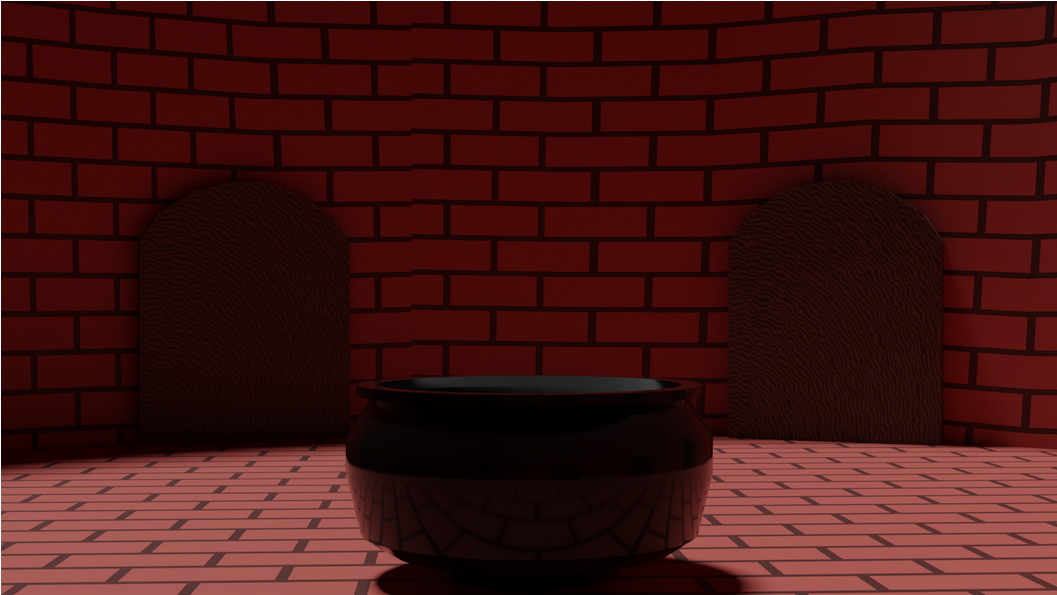
\includegraphics[width=300pt]{UserView.png}
  \caption{User view of the first level. Created in Blender. Assets by Sophia Girard (\url{https://drive.google.com/file/d/1gqC7niJWbHKXwep6VMvGeb8tZ0z4omwC/view?usp=share_link}).}
  \Description{Screenshot of virtual environment.}
\end{figure}

\begin{figure}[h]
  \centering
  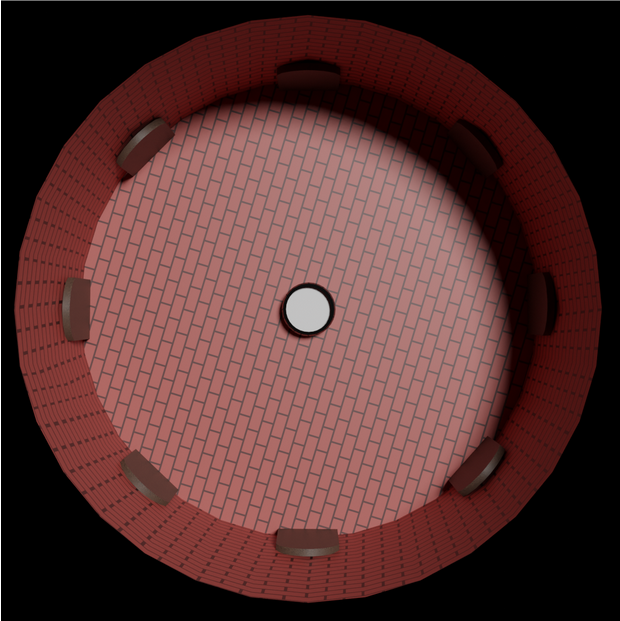
\includegraphics[width=250pt]{OverheadView.png}
  \caption{Bird's-eye view of the first level. Assets by Sophia Girard
  (\url{https://drive.google.com/file/d/12d1jHWMlpj5Wk3-TP-Q5hmh3d0j-AZ2X/view?usp=share_link}).}
  \Description{Screenshot of virtual environment.}
\end{figure}
\clearpage

Virtual Reality may be a useful medium to increase a person’s learning by helping to motivate and boost their confidence more than similar scenarios on a desktop. We studied a person’s motivation and confidence in completing a series of tasks in Virtual Reality versus on a desktop. We staged this study in an escape room solver program where we surveyed the participant on their confidence before and after and measured how quickly they solved the puzzle on the given platform.


%%
%% The next two lines define the bibliography style to be used, and
%% the bibliography file.
\bibliographystyle{ACM-Reference-Format}
\bibliography{bibliography}



\end{document}
\endinput
%%
%% End of file `sample-manuscript.tex'.
